\begin{figure}[tb]
\centering
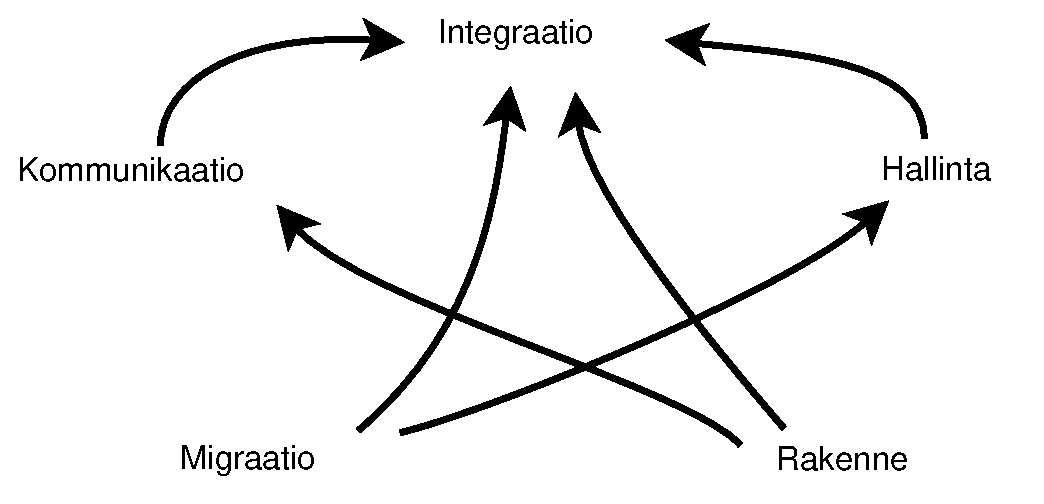
\includegraphics[scale=0.5]{riippuvuudet.eps}
\caption{Reuna-arkkitehtuurien ominaisuuksien yleiset riippuvuudet} \label{fig:riippuvuudet}
\end{figure}

\subsection{Vertailu}
Seuraavaksi käydään läpi edellä esitettyjen reunalasketa-arkkitehtuurien ominaisuuksia ja käsitellään niiden vaikutuksia itse toteutettavaan järjestelmään.
Kunkin arkkitehtuuriehdotuksen ominaisuusjoukko ohjaa toteutusta erilaisiin ratkaisuihin. Taulukoon \ref{table:features} on tiivistetysti koottu kunkin arkkitehtuuriratkaisun ominaisuudet.
Lopuksi käsitellään reuna-arkkitehtuurien yhteneväisyyksiä ja eroja ETSI:n MEC spesifikaation kanssa.

On tärkeää huomata, että käsiteltyjen ominaisuuksien välillä on riippuvuksia. Tämän seurauksena jonkin ominaisuuden toteuttaminen tietyllä tavalla saattaa estää tai rajoittaa joidenkin toiminnallisuuksien toteuttamista. 
Reuna-arkkitehtuurien keskeisin ominaisuus on tapa jolla järjestelmä integroituu osaksi mobiiliverkkoa. Kaikki muut ominaisuudet vaikuttavat olevan riippuvaisia siitä.
Kuvassa \ref{fig:riippuvuudet} on esitetty ominaisuuksien väliset riippuvuudet.
Rakenne on tyypiltään implisiittinen ominaisuus. Se ei siis pääsääntöisesti ole reuna-arkkitehtuurin määrittelemä, vaan sen toteutus on riippuvainen reuna-arkkitehtuurin muista ominaisuuksista.

Kappaleessa \ref{integraatio} esiteltyjen integraatiotyyppien jaon mukaan SCC ja CONCERT edustavat suoraa integraatiota, SMORE ja MobiScud edustavat läpinäkyvää integraatiota ja FMC edustaa epäsuoraa integraatiota.

SCC liittyy mobiiliverkon toimintoihin niin sanotusti natiivien yhteyksien avulla. Se edellyttää uusia rajapintoja mobiiliverkon nykyisiin komponentteihin. Tavoitteena on SCC:n hallinnollisten tarpeiden täyttämiseen. Lisäksi SCC edellyttää reunaresurssien integrointia osaksi tukiasemaa. 
Tukiasemaan sidottujen reunaresurssien vuoksi SCC:n rakenne on litteä. 
SCC:n mukaan uudistetun tukiaseman, eli SCeNBce:n, tehtäviin kuuluu reunapalveluille tarkoitetun tietoliikenteen ohjaaminen. Tämä tarkoittaa, että SCeNBce monitoroi tietoliikennettä ja ohjaa esimerkiksi kohde IP:n perusteella reunapalvelulle tarkoitetut paketit.

CONCERT on toinen suoran integraation reunajärjestelmä. Ehdotuksen tavoitteena on NFV:n laajamittainen käyttöönotto, jonka avulla mobiiliverkon ja reunajärjestelmä voisivat jakaa laskentaresursseja. Järjestelmä rakentuu kolmeen kerrokseen hierarkkisesti sijoitettujen resurssien varaan. Nämä resurssit ovat reunalaskennan ja mobiiliverkon toiminnallisuuksien käytettävissä. 
Mobiiliverkon ja reunalaskennan hallinnolliset toimet on yhdistetty Conductor nimiselle entiteetille. Conductor sisältää useita alitoimintoja, joiden tehtäviin kuuluu muun muassa resurssien jakaminen kullekkin toiminnallisuudelle. CONCERT ottaa hallinnollisiin tehtäviin kantaa ainoastaan yleisellä tasolla ja yksityiskohdat jätetään avoimeksi. Oletettavaa on että CONCERT:ssa mobiiliverkon ja reunajärjestelmän reititys tapahtuu samassa kontekstissa, jolloin järjestelmä ei vaadi erillistä toiminnallisuutta reunasolmuille suuntautuvan tietoliikenteen ohjaamiseen. 

MobiScud ja SMORE edustavat läpinäkyvää integraatiota.
SDN-kerros eNodeB ja EPC:n komponenttien välillä mahdollistaa tietoliikenteen monitoroinnin sekä ohjaamisen.
SDN-kerros keskeinen hyöty on mobiiliverkon nykyisten toimintojen säilyttämisen ennallaan.
Koska tietoliikenne reunaresursseille ohjataan SDN-kerroksen sisällä, reunasolmujen sijoittelu ei ole suoranaisesti riippuvaista mobiiliverkosta.  
Teoriassa reunasolmujen sijoittelu on täysin vapaa. 
SMORE ja MobiScud ehdottavat toisistaan poikkeavaa sijaintia reunasolmuille. SMORE:ssa yhdelle reunasolmulle klusteroidaan suuri joukko tukiasemia, kun taas MobiScud ehdottaa reunasolmujen sijoittelua yksittäisten tukiasemien läheisyyteen.
Tämä tarkoittaa että järjestelmät eroavat yksittäiseen reunasolmuun sijoitettavien laskentaresurssien määrältä huomattavasti.
SMORE:n tapauksessa yhden reunasolmun vastuualueeksi oletetaan niin suuri joukko tukiasemia, että laskennan siirrolle ei ole tarvetta, eli järjestelmä ei toteuta live migraatiota.
MobiScud puolestaan hajautetummilla resursseillaan edellyttää reunalaskennan siirtoa ja ehdottaakin sille toiminnallisuutta.
SMORE:n ja MobiScud:n yhteisenä ominaisuutena on mekaniikka, jolla tietoliikenne ohjataan reunasolmuille siten, että se ei vaikuta mobiiliverkon toimintaan.
Molemmissa ratkaisuissa SDN-kerros sisältää toiminnallisuuden, joka haarauttaa reunasolmuille tarkoitettua liikennettä monitoroimalla mobiiliverkon GTP-tunneleita.
Tarpeen mukaan GTP-tunneloitujen pakettien GTP paketointi puretaan ja välitetään SDN-kerroksen sisällä reunasolmulle. 
Samaa monitorointitoiminnallisuutta käytetään molemmissa ratkaisuissa myös mobiiliverkon kontrollitason seuraamiseen, joka mahdollistaa mobiiliverkon tapahtumiin reagoinnin.
MobiScud tekee reunalaskennan migraatioon liittyvät päätökset kontrollikerroksella ilmenevien tapahtumien kautta saatuihin tietoihin.
%
%Koska SDN-kerros sijaitsee eNodeB:n ja EPC:n välillä joudutaan asiakaslaitteen ja reunasolmun välistä liikennettä muokkaamaan. Kyseisellä välillä tietoliikenne on GTP tunneloitua.
%Riippuen onko paketti menossa reunasolmulle vai tulossa reunasolmulta, joudutaan tunnelointi purkamaan tai paketoimaan. Tämä saattaa johtaa merkittävään viiveeseen yhdessä monitoroinnin kanssa.
%MobiScudissa SDN-kerros sijaitsee eNodeB:n välittömässä läheisyydessä, kun taas SMORE:ssa sen oletetaan sijaitsevan useamman eNodeB:n yhteyspisteessä. 

Ainoa epäsuoraa integraatiota edustava ratkaisu on FMC.
FMC:n tavoitteena on viedä mobiiliverkon yhteydet nopeammin ulkoverkossa sijaitseville palvelinresursseille. Mobiiliverkon ulkopuolelle sijoitetut resurssit mahdollistavat sen että reunajärjestelmää voi ylläpitää jokin ulkoinen taho.
FMC ei siis suoranaisesti ota kantaa tapaan jolla reunaresurssit on järjestetty. Mutta on perusteltua olettaa että ne sijaitsisivat mobiiliverkon P-GW yhdyskäytävien läheisyydessä.
FMC:n tapa mahdollistaa reunapalvelun ja asiakaslaitteen välinen kommunikaatio perustuu sessiotunnistesiin. Se mahdollistaa asiakaslaitteen ja reunpalvelun IP-osoitteiden vaihtumisen, ilman että viitteet asiakaslaitteen ja reunapalvelun välillä katkeavat. Järjestelmä ei siis edellytä tavallisesta poikkeavaa mekaniikkaa tietoliikenteen reitittämiseksi. Ainoa edellytys on asiakaslaitteen sovellukseen sekä reunapalvelun toiminnallisuuden ohjelmallisen toimijan joka huolehtii yhteyksien varmistamisesta sessiotunnisteiden avulla.

Myös hallinnollisten toimien toteuttaminen on osittain riippuvaista integraatiosta. Suoran integraation järjestelmissä hallinnollisella entiteetillä on oma rajapinta mobiiliverkon toimintojen kanssa. 
Toisaalta se edellyttää olemassa olevaan järjestelmään rajapinnan toteuttamisen, mutta lisäksi tarjoaa helpon keinon tehdä hallinnollisia toimia mobiiliverkon sisällä. 
Läpinäkyvässä järjestelmässä hallinnollinen entiteetti on riippuvainen mobiiliverkon viestien monitoroinnin kautta saatavasta tiedosta. 
MobiScud ja SMORE tarkkailevat SDN-kerroksen avulla mobiiliverkon kontrollitason viestintää. 
Vaikka läpinäkyvät integraatiot ovat loogisesti erillään mobiiliverkosta, edellyttävät ne pääsyä mobiiliverkon sisäisiin tietoliikenneväyliin.
Täten todennäköisintä on että järjestelmää ylläpitää mobiiliverkon operaattori eikä ulkoinen taho. 
Epäsuoraa integraatiota edustavassa FMC:ssä hallinnolliset toiminnot edellyttävät tietoja mobiiliverkosta. Tieto on tyypiltään staattista, joten aktiivista tiedosiirtoa mobiiliverkon ja FMC:n välille ei tarvita.
Edellytyksenä on esimerkiksi taulukko, josta voidaan lukea asiakaslaitteen IP-osoittetta vastaava fyysinen alue tai P-GW:n sijainti. Tämä mahdollistaa FMC:n ohjata asiakaslaitteen yhteys lähimmälle palvelinsalille. 


SMORE, MobiScud ja FMC esittelevät toiminnot, joilla asiakaslaitteen liikkumisesta seuraavat yhteysmuutokset otetaan huomioon reunajärjestelmässä.
Varsinaiseen reunapalvelun siirtämiseen oletetaan live migraation kaltainen mekanismi lähes kaikissa ehdotuksissa. Ainoastaan SMORE olettaa reunasolmun sijaitsevat niin keskeisessä yhteyspisteessä, että reunapalveluiden siirtelylle ei ole tarvetta.
Tällä arkkitehtuuritasolla ei ole kannattavaa ottaa kantaa reuna-alustan tehtäviin, koska se rajoittaisi arkkitehtuurin sovellettavuutta erilaisten reunapalveluiden tarjoamiseen.

\begin{landscape}
    \noindent
\begin{table}[!ht]
\caption{Reunalaskenta-arkkitehtuurien ominaisuudet tiivistetysti}
\label{table:features}
\begin{tabularx}{ \hsize }{ | c | c | c | p{3cm} | c | X | }
\hline 
 \textbf{Ominaisuus} & \textbf{Integraatio} & \textbf{Rakenne} & \textbf{Migraatio} & \textbf{Hallinta} & \textbf{Kommunikaatio} \\ 
\hline 
 FMC & Epäsuora & Vapaa & Palveluiden siirto ulkopuolisten salien välillä & FMC Controller & Tavalliset reititys, mutta palveluiden ja asiakaslaitteen yhdistämiseen erillinen sessiotunniste \\ 
\hline 
 SMORE & Läpinäkyvä & Vapaa & Ei sisällä & SMORE Controller & SDN monitori ja reititys \\ 
\hline 
MobiScud & Läpinäkyvä & Vapaa & Live migraatio & MobiScud Controller & SDN monitori ja reititys\\ 
\hline 
SCC & Suora & Litteä & Live migraatio & SCM & Monitori ja reititys tukiasemassa \\ 
\hline 
CONCERT & Suora & Hierarkkinen & Live migraatio & Conductor & SDN reititys mobiiliverkossa \\ 
\hline 
\end{tabularx} 
\end{table}
\end{landscape}

\subsubsection{Yhteensopivuus ETSI MEC vaatimuksiin}

%Yleiset periaatteet ja vaatimukset
ETSI MEC spesifikaation teknisiä vaatimuksia esittelevä dokumentti \cite{etsitechreq} määrittelee reunalaskennalle yleiset periaatteet ja konkreettisemmin määriteltyjä toiminnallisia vaatimuksia. 
Yleiset periaatteet ovat korkean tason tavoitteita reunajärjestelmälle.
Reuna-arkkitehtuurien kannalta merkityksellisimmät periaatteet ovat NFV yhteensopivuus, liikkuvuuden tukeminen ja käyttöönoton riippumattomuus.
Toiminnallisuudet vaatimukset on jaettu useampaan kategoriaan, jotka esiteltiin kappaleessa \ref{etsi}.
Ainoastaan osa toiminnallisista vaatimuksista on relevantteja arkkitehtuureja tarkasteltaessa ja suurin osa näistä vaatimuksista koskee reuna-alustan ohjelmallisia toimijoita, joihin ei reuna-arkkitehtuureissa oteta kantaa.
Lisäksi suurin osa vaatimuksista on ainoastaan täsmennyksiä yleisiin periaatteisiin.
Seuraavaksi käydään läpi yleisten periaatteiden toteutuminen ehdotetuissa reuna-arkkitehtuureissa.

Tässä tukielmassa käsiteltyjen reuna-arkkitehtuurien yhteydessä ei esiintynyt NFV yhteensopivuutta rajoittavia tekijöitä. Eli kaikki käsitellyt arkkitehtuurit olivat pääsääntöisesti NFV yhteensopivia.
CONCERT oli ainoa reuna-arkkitehtuuri joka nimenomaisesti rakentui NFV:n varaan. Muissa arkkitehtuureissa NFV:tä pidettiin enemmänkin mahdollisuutena.
Esimerkiksi SCC:n yhteydessä esitettiin, että tukiasemaan sidottuja resursseja voisi käyttää myös tukiasemien omien toimintojen tuottamiseen NFV:n avulla. 


Perinteisesti mobiiliverkoissa liikkuvuuden tukeminen tarkoittaa, että handover tapahtumat eivät ilmene asiakaskerroksella, esimerkiksi puheluissa ja tietoliikenneyhteyksissä.
Samaa palveluvaatimusta on luonnollista olettaa myös reunajärjestelmältä. 
Käytännössä reunajärjestelmän tulee vähintää ylläpitää asiakaslaitteen ja reunapalvelun välistä yhteyttä.
Tämän lisäksi palvelun laadun takaamiseksi kyseeseen tulee myös reunapalveluiden siirto.
Liikkuvuuden tukeminen reunajärjestelmissä koostuu siis yhteyden ylläpidosta ja reunapalveluiden siirtelystä.
Tässä tukielmassa SMORE, MobiScud ja FMC esittivät mekanismin yhteyden ylläpitämiseksi asiakaslaitteen liikkuessa verkossa.
SMORE ja MobiScud toteuttivat yhteyden ylläpitämisen SDN reititysmuutoksilla.
FMC puolestaan nojaa erilliseen sessiotunnisteeseen, joka häivyttää IP-osoitteiden muutokset.
Lähes kaikki reuna-arkkitehtuurit tiedostivat tarpeen reunapalveluiden siirtelyn tarpeelle.
SMORE:a lukuunottamatta kaikki arkkitehtuurit olettivat virtuaalikoneiden live migraatiota jossain muodossa.  
ETSI:n MEC referenssiarkkitehtuuri olettaa reunajärjestelmän toteuttavan Cloudlet VM handoff kaltaista toiminnallisuutta \cite{etsirefarch}.
On kuitenkin täysin reunapalveluiden tyypistä riippuvaista, kuinka liikkuvuuteen on kannattavaa reagoida \cite{etsitechreq}. 

Reunajärjestelmän yleisiin periaatteisiin kuuluu käyttöönoton riippumattomuus (deployment independence) \cite{etsitechreq}.
Käyttöönoton riippumattomuudella tarkoitetaan, että reunajärjestelmän käyttöönottajalla olisi mahdollisuus sijoitella reunajärjestelmän osat omien vaatimuksiensa mukaan \cite{etsitechreq}. Pääasiassa tämä koskee reunasolmujen sijoittelua. Tässä tutkielmassa reunasolmujen sijoittelua on käsitelty implisiittisenä ominaisuutena, jonka määrittelevinä ominaisuuksina toimivat integraation tyyppi ja kommunikaatio. 
Teoriassa eniten vapauksia reunajärjestelmän toteuttamiseen tarjoavat läpinäkyvää integraatiota toteuttavat SMORE ja MobiScud.
Nämä järjestelmät edellyttävät ainoastaan yhden yhteyspisteen mobiiliverkkoon ja ovat muuten täysin vapaasti järjesteltävissä.
Suoran integraation reuna-arkkitehtuureissa edellytetään jotain tiettyä rakennetta. 
SCC edellyttää reunaresurssien sijoittamisen tukiasemiin. SCC kuitenkin loogisesti erottaa reunajärjestelmän ja mobiiliverkon haarauttamalla reunapalveluille tarkoitetun tietoliikenteen erillisellä monitoritoiminnallisuudella.
Toinen suoraa integraatiota edustava järjestelmä, CONCERT, edellyttää hierarkista asettelua reunaresursseille. CONCERT:n NFV painotteisuus kuitenkin takaa toiminnallisuuksien vapaan sijoittelun. CONCERT tarjoaa SCC:hen verrattuna enemmän vapauksia resurssien sijoitteluun.
FMC, ainoana epäsuorana itengraationa, tarjoaa myös vapauden sijoitella reunajärjestelmän, mutta ainoastaan mobiiliverkon ulkopuolelle.
FMC:tä ei siis voi pitää erityisen riippumattomana, koska reunapalveluita tarjoavat resurssit joudutaan sijoittelemaan pakettiverkon yhdyskäytävien läheisyyteen.

%Referenssi-arkkitehtuuri


%ETSI MEC spesifikaatio edellyttävät reunajärjestelmältä tiettyjä ominaisuuksia.
%Seuraavaksi käsitellään tässä tutkielmassa esiteltyjen reuna-arkkitehtuurien kykyä vastata näihin vaatimuksiin.
%ETSI MEC spesifikaatio käsittelee reunalaskentaa korkealla tasolla, eikä siis ota kantaa teknisiin toteutuksiin.
%%Spesifikaatio asettaa vaatimuksia sekä tarjoaa mahdollisuuksia.
%ETSI MEC tekniset vaatimukset \cite{etsitechreq} on jaettu yleisiin periaatteisiin ja vaatimuksiin.
%
%Yleisien periaatteiden reuna-arkkitehtuurien kannalta tärkeät osuudet ovat NFV yhteensopivuus, liikkuvuuden tukeminen ja käyttöönoton riippumattomuus.
%T
%
%Mobiiliverkoissa liikkuvuuden (mobility) tukeminen tarkoittaa, että handover tapahtumat eivät mobiiliverkkoa käyttäessä näy asiakaskerroksella, esimerkiksi puheluissa ja tietoliikenneyhteyksissä.
%Täten samaa palveluvaatimusta oletetaan myös mobiiliverkossa toimivalta reunalaskennalta.
%Tämä tarkoittaa että reunalaskennan tulee reagoida asiakaslaitteen liikkumiseen verkossa, jotta voidaan varmistaa palvelun jatkuminen.
%Liikkuvuuden tukeminen tarkoittaa reuna-arkkitehtuureissa reunalaskennan siirtoa ja yhteyden päivittämistä.
%Kaikki järjestelmät tukevat tätä, mutta yksityiskohdissa on eroa.
%Mitään erityistä palvelun laadullista vaatimusta ei ole ETSI:n teknisten vaatimusten dokumenteissa asetettu, mutta osa reuna-arkkitehtuureista on ottanut lähtökohdakseen että pelkkä yhteyden ylläpitäminen reunalaskentaan ei riitä vaan sen tulee myös seurata asiakaslaitetta paremman palvelun laadun takaamiseksi.
%
%
%Liikkuvuuden tukeminen tarkoittaa mobiiliverkkojen kontekstissa asiakaslaitteen handoverin tukemista. 
%
%Reunalaskennan siirtäminen on pääasiassa tuettuna live migraation avulla. 
%
%Käyttöönoton riippumattomuus esittää että reunajärjestelmän tulee tukea erilaisia variaatioita käyttöönotolle.
%Tämä tarkoittaa esimerkiksi reunasolmujen sijoittelun tulisi olla täysin järjestelmän rakentajan valittavissa. 
%SCC on ainoa esitellyistä reuna-arkkitehtuureista, joka pakottaa reunaresurssien sijoittamisen tukiasemaan.
%MobiScud ja SMORE ehdottavat reunasolmuille sijainnit, mutta integraation tyylistä johtuen sijoittelu on käytännössä vapaa. 
%FMC tarjoaa myös vapauden sijoitella reunasolmuja, mutta ainoastaan mobiiliverkon ulkopuolelle. 
%CONCERT eroaa muista ehdotuksista ehdottamalla kolmiportaista hierarkkiaa reunalaskennan resursseille.
%Johtuen CONCERT:n NFV painotteisuudesta fyysisiä reunasolmuja ei ole, vaan resurssit ovat vapaasti mobiiliverkon ja reunajärjestelmän käytettävissä. 
%CONCERT:n tapauksessa reunapalveluiden sijoitteluun on siis mahdollista vaikuttaa ohjelmistotasolla.
%
%
%Koska osa spesifikaatiosta käsittelee palvelun tuottamiseen liittyviä vaatimuksia, on niiden käsittely mahdollista ainoastaan niiltä osin kuin ne eivät koske reunapalveluiden tyyppejä.
%Vaatimuksien osalta Mahdollistaa tai ei mahdollista
%Tässä tutkielmassa esitettyjen reuna-arkkitehtuurien osalta vertailu

%=========



%Reuna-arkkitehtuurien ominaisuuksien vertailu aloitetaan live migraatiosta.
%\par
%Live migraatio on toiminnallisuuksista se joka mahdollistaa suurempien palvelukokonaisuuksien siirtämisen reunajärjestelmässä. Syitä reunalaskennan siirtämiselle voi olla useita ja ehkä yleisin pinnalle noussut syy on asiakaslaitteen liikkuminen verkossa. Muita syitä live migraatiolle voi olla esimerkiksi laskennan siirtäminen enemmän resursseja sisältävälle reunapalvelulle tai ylikuormituksen välttäminen nykyisellä reunasolmulla.
%%migraatio edellyttää reunasolmujen olemista samalla palveluntarjoajalla.
%
%Live migraatio toiminnallisuuden puuttumisen voi tulkita ainakin kahdella tavalla. Joko se tarkoittaa, että reunalaskenta on muodoltaa etälaskentaa, joka on niin hienojakoista, että migraatiolle ei ole tarvetta. Tällöin etälaskenta rajoittuu pieniin työyksiköihin joista odotetaan välitöntä tulosta asiakaslaitteelle. 
%Toinen vaihtoehto on että tarjolla olevat reunasovellukset ovat tyypiltään yleiskäyttöisiä, esimerkiksi pelipalvelimia.
%
%Lähes kaikki reuna-arkkitehtuurit tiedostivat tarpeen live migraatiolle. Ainoastaan SCC ei sisältänyt edes mainintaa reunasovelluksien siirtelystä reunasolmulta toiselle.
%
%
%\par
%Reuna-arkkitehtuurin kommunikaatio
%
%\par
%Reuna-arkkitehtuurin 
%

% Taulukko toiminnoista
